\chapter{Halbleitertechnologien}
Jedes PE, egal ob ISP, ASIP oder ASP muss gefertigt werden. Hierfür muss sich für eine Herstellungsart entschieden werden.
\begin{figure}[H]
    \centering
    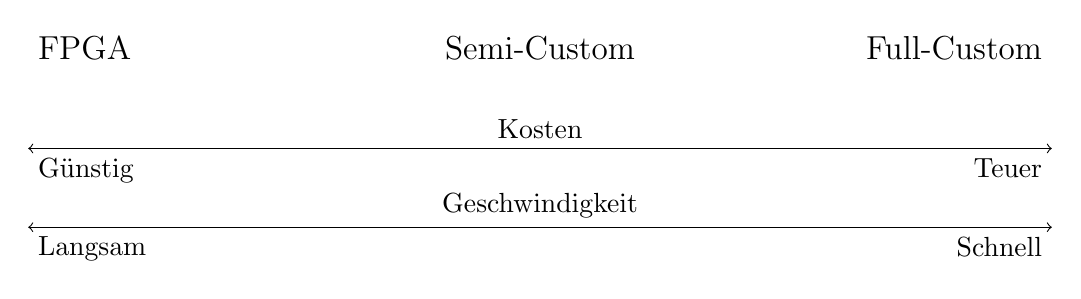
\begin{tikzpicture}
        \draw[<->] (0,0) -- (13,0) node[above, pos=.5] {Geschwindigkeit};
        \node[below right] at (0,0) (){Langsam};
        \node[below left] at (13,0) (){Schnell};
        \draw[<->] (0,1) -- (13,1) node[above, pos=.5] {Kosten};
        \node[below right] at (0,1) (){Günstig};
        \node[below left] at (13,1) (){Teuer};
        \node[above right] at (0,2) (){\large{FPGA}};
        \node[above] at (6.5,2) (){\large{Semi-Custom}};
        \node[above left] at (13,2) (){\large{Full-Custom}};
    \end{tikzpicture}
    \caption{Optionen für die fertigung von Halbleiterkomponenten}
\end{figure}

\begin{figure}[H]
    \centering
    \includegraphics[width=\textwidth]{ic.pdf}
    \caption{Überblick über ICs}
\end{figure}

\section{Full-Custom-Logic Fabric}
Sehr teuer, dafür aber maximale Performance. 
Lohnt sich im Normalfall nur für sehr große Stückzahlen.
Beispiele für Full-Custom gefertigte Komponenten:
\begin{itemize}
    \item PC-Processoren
    \item GPUs
    \item ASIPs (z.b. Basisbandprozessoren)
    \item Microcontroller
\end{itemize}

Üblicherweise werden Full-Custom-Komponenten in \glqq{}complementary metal-oxide-semiconductor\grqq{} (CMOS) Technik gefertigt.

\section{Semi-Custom (Gate-Array)}
Ein Gate-Array besteht aus vielen, nicht verbundenen, Transistorzellen, sogenannten Basismakros. 
Vom Anwender kann sowohl die Funktion jeder Logikzelle (NAND oder NOR) sowie die Verbindungen zwischen den Logikzellen bestimmt werden.
Semi-Custom-Komponenten sind deutlich größer als Full-Custom-Komponenten.
\begin{figure}[H]
    \centering
    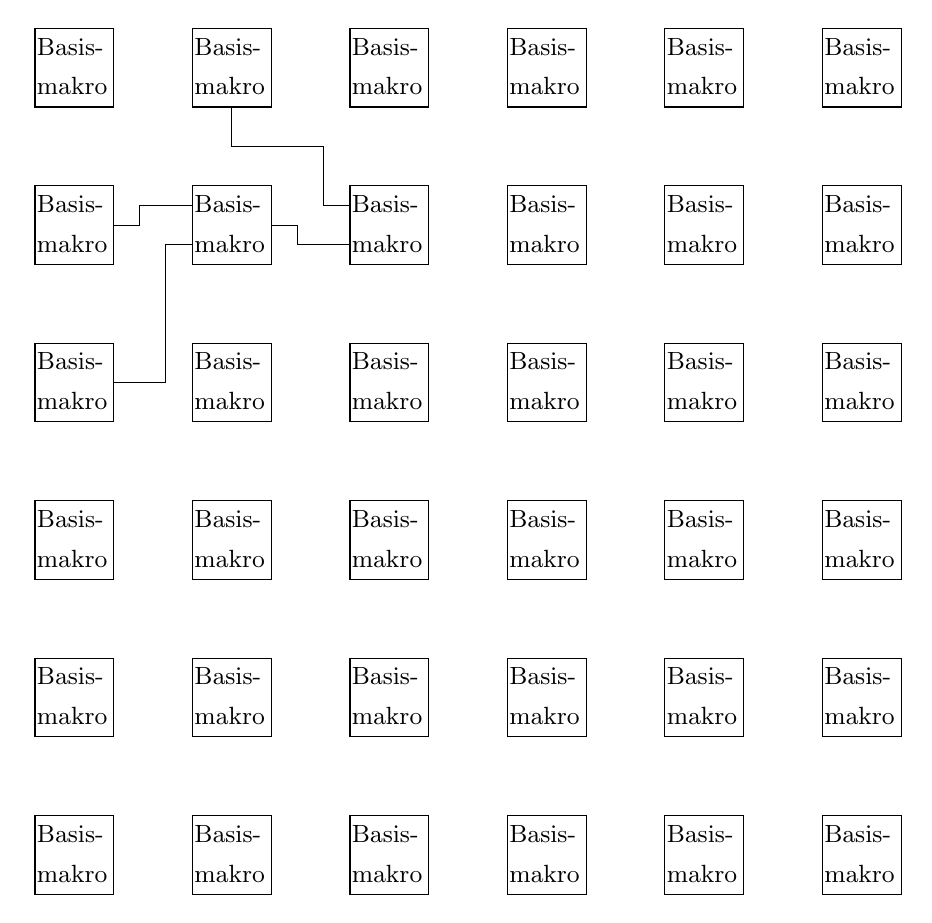
\begin{tikzpicture}
        \foreach \i in {0,...,35}
        {
            \pgfmathtruncatemacro{\y}{\i / 6};
            \pgfmathtruncatemacro{\x}{\i - 6*\y};
            \ifthenelse{\x=0 \OR \x=5 \OR \y = 0 \OR \y=5}{
                \filldraw [draw=black,fill=gray!40] (\x*2,\y*2) rectangle (\x*2+1,\y*2+1);
                \node[below right] at (\x*2,\y*2+1) (){\small{Pad}};
            }{
                \filldraw [draw=black,fill=white] (\x*2,\y*2) rectangle (\x*2+1,\y*2+1);
                \node[below right] at (\x*2-0.1,\y*2+1) (){\small{Basis-}};
                \node[below right] at (\x*2-0.1,\y*2+0.5) (){\small{makro}};
            }
        }
        \draw (1,8.5) -| (1.33,8.75) -| (2,8.75);
        \draw (1,6.5) -| (1.66,8.25) -| (2,8.25);
        \draw (3,8.5) -| (3.33,8.25) -| (4,8.25);
        \draw (2.5,10) |- (3.66,9.5) |- (4,8.75);
    \end{tikzpicture}
    \caption{Aufbau eines Gate-Arrays}
\end{figure}

\begin{figure}[H]
    \begin{subfigure}[b]{.2\textwidth}
        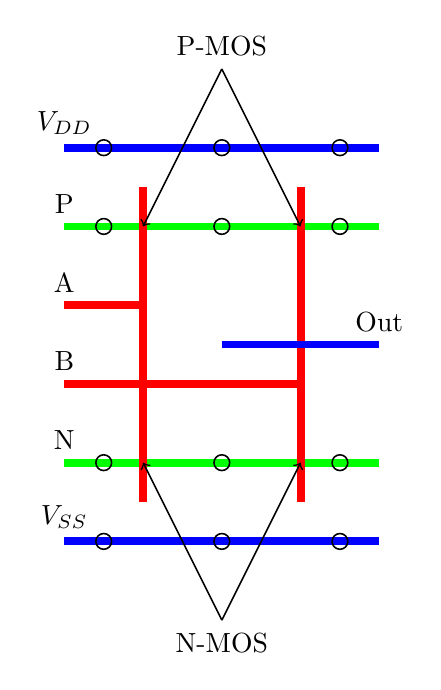
\begin{tikzpicture}[line width=0.1cm]
            \draw[draw=blue] (0,5) -- (4,5) node[above,pos=0]{$V_\text{DD}$};
            \draw[draw=blue] (0,0) -- (4,0) node[above,pos=0]{$V_\text{SS}$};
            \draw[draw=green] (0,4) -- (4,4) node[above,pos=0]{P};
            \draw[draw=green] (0,1) -- (4,1) node[above,pos=0]{N};
            \draw[draw=red] (1,0.5) -- (1,4.5);
            \draw[draw=red] (3,0.5) -- (3,4.5);
            \draw[draw=red] (0,3) -- (1,3) node[above,pos=0]{A};
            \draw[draw=red] (0,2) -- (3,2) node[above,pos=0]{B};
            \draw[draw=blue] (2,2.5) -- (4,2.5) node[above,pos=1]{Out};
            \foreach \x in {0.5,2,3.5} {
                \foreach \y in {0,1,4,5} {
                    \draw[line width=0.02cm] (\x,\y) circle (0.1cm);
                }
            }
            \draw[line width=0.02cm,->] (2,6) -- (1,4);
            \draw[line width=0.02cm,->](2,6) -- (3,4);
            \node[above] at (2,6) (){P-MOS};
            \draw[line width=0.02cm,->] (2,-1) -- (1,1);
            \draw[line width=0.02cm,->](2,-1) -- (3,1);
            \node[below] at (2,-1) (){N-MOS};
        \end{tikzpicture}
        \subcaption{Nicht konfigurierte Basiszelle als \glqq{}offener Inverter\grqq{}}
    \end{subfigure}
    \hfill
    \begin{subfigure}[b]{.2\textwidth}
        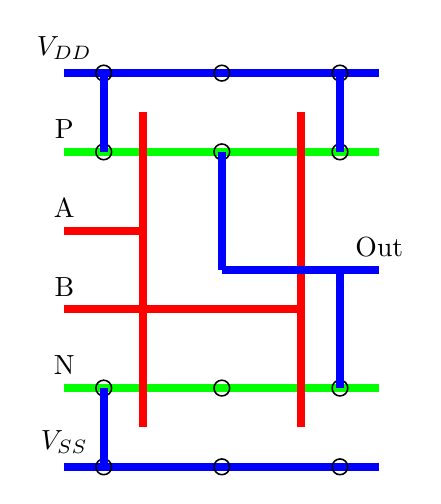
\begin{tikzpicture}[line width=0.1cm]
            \draw[draw=blue] (0,5) -- (4,5) node[above,pos=0]{$V_\text{DD}$};
            \draw[draw=blue] (0,0) -- (4,0) node[above,pos=0]{$V_\text{SS}$};
            \draw[draw=green] (0,4) -- (4,4) node[above,pos=0]{P};
            \draw[draw=green] (0,1) -- (4,1) node[above,pos=0]{N};
            \draw[draw=red] (1,0.5) -- (1,4.5);
            \draw[draw=red] (3,0.5) -- (3,4.5);
            \draw[draw=red] (0,3) -- (1,3) node[above,pos=0]{A};
            \draw[draw=red] (0,2) -- (3,2) node[above,pos=0]{B};
            \draw[draw=blue] (2,2.5) -- (4,2.5) node[above,pos=1]{Out};
            \foreach \x in {0.5,2,3.5} {
                \foreach \y in {0,1,4,5} {
                    \draw[line width=0.02cm] (\x,\y) circle (0.1cm);
                }
            }
            \draw[blue] (0.5,4) -- (0.5,5);
            \draw[blue] (3.5,4) -- (3.5,5);
            \draw[blue] (0.5,0) -- (0.5,1);
            \draw[blue] (2,4) -- (2,2.5);
            \draw[blue] (3.5,1) -- (3.5,2.5);
        \end{tikzpicture}
        \subcaption{NAND}
    \end{subfigure}
    \hfill
    \begin{subfigure}[b]{.2\textwidth}
        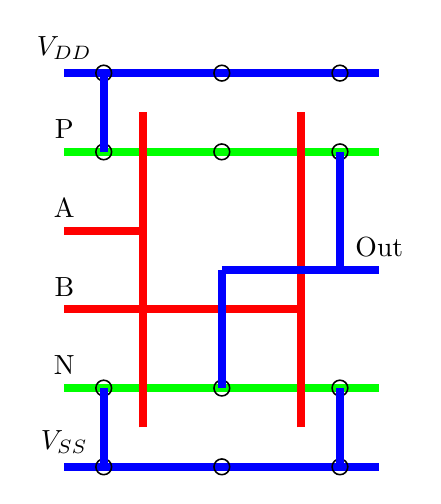
\begin{tikzpicture}[line width=0.1cm]
            \draw[draw=blue] (0,5) -- (4,5) node[above,pos=0]{$V_\text{DD}$};
            \draw[draw=blue] (0,0) -- (4,0) node[above,pos=0]{$V_\text{SS}$};
            \draw[draw=green] (0,4) -- (4,4) node[above,pos=0]{P};
            \draw[draw=green] (0,1) -- (4,1) node[above,pos=0]{N};
            \draw[draw=red] (1,0.5) -- (1,4.5);
            \draw[draw=red] (3,0.5) -- (3,4.5);
            \draw[draw=red] (0,3) -- (1,3) node[above,pos=0]{A};
            \draw[draw=red] (0,2) -- (3,2) node[above,pos=0]{B};
            \draw[draw=blue] (2,2.5) -- (4,2.5) node[above,pos=1]{Out};
            \foreach \x in {0.5,2,3.5} {
                \foreach \y in {0,1,4,5} {
                    \draw[line width=0.02cm] (\x,\y) circle (0.1cm);
                }
            }
            \draw[blue] (0.5,1) -- (0.5,0);
            \draw[blue] (3.5,1) -- (3.5,0);
            \draw[blue] (0.5,4) -- (0.5,5);
            \draw[blue] (2,1) -- (2,2.5);
            \draw[blue] (3.5,4) -- (3.5,2.5);
        \end{tikzpicture}
        \subcaption{NOR}
    \end{subfigure}
    \caption{Aufbau und Nutzung der Transistorzellen/Basismakros}
\end{figure}

\section{Programmierbare Schaltungen (Programmable Gate Fabric)}
Ziel: Logikelemente selbst verbinden $\Rightarrow$ Schaltelemente

Hinweis: Auch Logikelemente selber können konfigurierbar sein.

\begin{figure}[H]
    \centering
    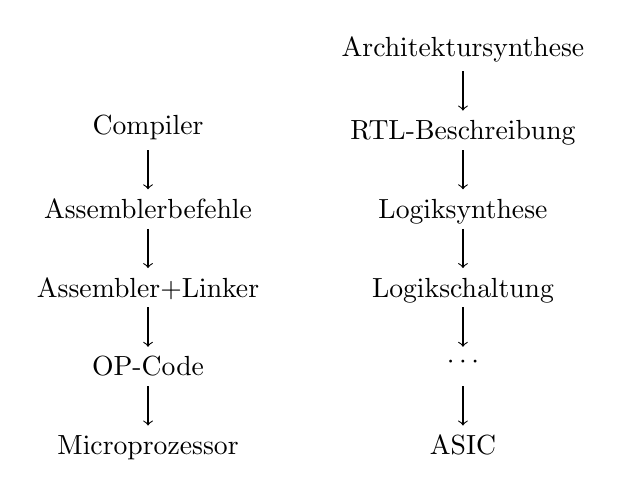
\begin{tikzpicture}
        \draw[->] (0,1) -- (0,0.5) node[below]{Microprozessor};
        \draw[->] (0,2) -- (0,1.5) node[below]{OP-Code};
        \draw[->] (0,3) -- (0,2.5) node[below]{Assembler+Linker};
        \draw[->] (0,4) -- (0,3.5) node[below]{Assemblerbefehle};
        \node[above] at(0,4) (){Compiler};
        \draw[->] (4,1) -- (4,0.5) node[below]{ASIC};
        \draw[->] (4,2) -- (4,1.5) node[below]{$\cdots$};
        \draw[->] (4,3) -- (4,2.5) node[below]{Logikschaltung};
        \draw[->] (4,4) -- (4,3.5) node[below]{Logiksynthese};
        \draw[->] (4,5) -- (4,4.5) node[below]{RTL-Beschreibung};
        \node[above] at(4,5) (){Architektursynthese};
    \end{tikzpicture}
    \caption{Vergleich von Hardwarebeschreibung und \glqq{}normaler\grqq{} Software}
\end{figure}

\subsection{Programmable Logic Devices (PLDs)}
\begin{itemize}
    \item 3 Klassen:
        \begin{itemize}
            \item SPLD (Simple Programmable Logic Device)
            \item CPLD (Complex Programmable Logic Device)
            \item FPGA (Field Programmable Gate Array)
        \end{itemize}
    \item 2 Ebenen: \todo{Was  heißt das jetzt?}
        \begin{itemize}
            \item Funktionale Ebene (Logistrukturen)
            \item Konfigurationsebenen
        \end{itemize}
    \item Verbindungen werden über eine SRAM-Zelle geschaltet
        \begin{figure}[H]
            \centering
            \begin{circuitikz}
                \draw (1,3) node[nmos,rotate=-90] (left){};
                \draw (3,4) node[pmos,rotate=180] (lp){};
                \draw (6,4) node[pmos,rotate=0] (rp){};
                \draw (3,2) node[nmos,rotate=180] (ln){};
                \draw (6,2) node[nmos,rotate=0] (rn){};
                \draw (9,1) node[nmos,rotate=-45] (right){};
                \draw (left.C) |- (3,3);
                \draw (lp.E) |- (ln.E);
                \draw (rp.C) |- (rn.C);
                \draw (lp.C) |- (rp.E);
                \draw (ln.C) |- (rn.E);
                \draw (3,3) to[short,-*] (3,3);
                \draw (lp.B) |- (ln.B);
                \draw (rp.B) |- (rn.B);
                \draw (3,3.3) to[short,*-*] (5,3.3);
                \draw (4,2.7) to[short,*-*] (6,2.7);
                \draw (6,3) to[short,*-] (6,3);
                \draw (6,3) -| (right.B);
                \draw (0,0) -- (0,5);
                \draw (0,3) to[short,*-] (left.E);
                \draw (4.5,1.275) to[short,*-] (4.5,1) node[rground]{};
                \draw (4.5,4.775) to[short,*-] (4.5,5) node[vcc]{};
                \draw (10,-1) -- (10,5);
                \draw (7,0) -- (11,0);
                \draw (right.E) -| (8,0);
                \draw (right.C) |- (10,2);
                \draw (8,0) to[short,-*] (8,0);
                \draw (10,2) to[short,-*] (10,2);
            \end{circuitikz}
            \caption{SRAM-Zelle in einem PLD}
        \end{figure}
    \item Problem mit SRAM: Speicher ist flüchtig
    \item Alternativen: EPROM, EEPROM, Flash \todo{Bild Flash}
    \item Einmalige Programmierung (Anti-Fuse) \todo{Grafik}
\end{itemize}

\subsubsection{SPLDs}
Mögliche Formen von SPLDs sind:
\begin{itemize}
    \item PLA: Und und Oder Matrix, beide Programmierbar
    \item PROM: Und festverdrahtet, Oder Programmierbar (nicht jede Boolsche-Funktion abbildbar)
    \item PAL: Und Programmierbar, Oder fix
\end{itemize}
\todo{Grafik}

\subsubsection{CPLDs}
Viele Funktionsblöcke, dazwischen \glqq{}Fast Connect Switch Matrix\grqq{}.
\todo{Grafik}

\subsubsection{FPGAs}
Beliebige Logikfunktionen darstellbar durch Look-Up-Table (LUT).
\todo{Grafik}
\paragraph{Slice (kleinster Baustein)}
Ein Slice besteht aus zwei LUTs, zugehöriger Carry-Logik um Slices effizienter nacheinander zu schalten, sowie zwei Flip-Flops. 
\todo{Grafik}

\paragraph{Makro Cell (bei Xilinx: Configurable Logic Block, CLB)}
Eine Makro Cell wird über ein Bus-Netzwerk (vgl. Tiled-Architecture) angeschlossen.
\todo{Grafik}
